\chapter{Higgs Phenomenology at the LHC}
\label{sec:pheno}
\chaptermark{Higgs Phenomenology at the LHC}

\begin{center}
\begin{footnotesize}
{\it{``My drawing was not a picture of a hat. It was a picture of a boa constrictor digesting an elephant. Then, I drew the inside of the boa constrictor, so that the grown-ups could see it clearly. They always need to have things explained."}}\\
``Le Petit Prince", Antoine de Saint-Exup\'ery
\end{footnotesize}
\end{center}

\section{How to Find a Higgs at LHC}
\label{sec:LHCHiggs}

Just as with any other unstable particle in the Standard Model, when the LHC reaches a sufficient energy, the Higgs should be produced and then decay. Prior to discovery, it was known that if a SM Higgs boson existed, its production and decay must obey certain characteristics. By close examination of the decay products in CMS, we can pull back the curtain to see if a Higgs is hiding in one of these decay channels and if it matches the predictions of the Standard Model.

\subsection{An Interlude on Feynman Diagrams}
\label{sec:FeynDiagrams}

Before moving to specifics on how the Higgs is produced and decays at the LHC, we must diverge briefly to discuss production and decay more generally. Up to this point, we have been describing interactions in broad strokes, without delving into explicit mathematics. For the most part, we can continue without evaluating every integral and exponent, but these calculations still impact any analysis so we must find a way to encode these details. Fortunately, such a framework exists to represent the complicated mathematics behind the interactions of the Standard Model: \textit{Feynman Diagrams}. (Fig.~\ref{fig:FeynExample})

\begin{figure}[htbp]
\begin{center}
\unitlength=1mm
\begin{fmffile}{Phenomenology/figures/ComptonScattering}
\begin{fmfgraph*}(40,40)
  \fmfleft{i1,i2} \fmfright{sp1,sp2}
  \fmf{fermion,label=$e^+$}{i1,v1,sp1}
  \fmf{fermion,label=$e^+$}{i2,v2,sp2}
  \fmf{photon,label=$\gamma$}{v1,v2}
\end{fmfgraph*}
\end{fmffile}
\caption[Compton Scattering as an Example Feynman Diagram]{Compton Scattering as an example Feynman Diagram. With time going forward from left to right, two electrons approach each other, scatter via exchange of a photon, then move apart.}
\label{fig:FeynExample}
\end{center}
\end{figure}


In the most naive terms, particle physics measurements can be reduced to one goal: given initial particle states, what is the probability of producing a particular set of final particle states? As previously discussed in Sec.~\ref{sec:LHC}, the cross section of an event quantifies this probability, but it must be calculated somehow. In quantum field theories, the mathematical operation to convert incoming particle states to outgoing states via allowed operations of the model is the \textit{S-matrix}. Embedded in this matrix is the \textit{scattering matrix element} (commonly shortened to matrix element), $\mathcal{M}$, which encodes the full details of the interactions of a particular theory. The heuristic approach used to calculate the matrix element comes from summing the evaluations of all possible fully-connected\footnote{To be fully-connected, all incoming and outgoing particles must interact. In the calculation, these diagrams must also be amputated: self-interactions for a single particle do not, by definition, interact with the other particles and thus any diagrams with these elements do not contribute.} Feynman diagrams. Finally, the cross section is dependent upon the modulus squared\footnote{In general, a matrix element can be complex. As with other quantities in quantum mechanics, the modulus squared of an amplitude (e.g. the amplitude multiplied by its complex conjugate) will lead to measurable quantities. This also allows for the possibility of interference between different amplitudes.} matrix element which can be evaluated from the Feynman diagrams according to the rules of the interactions in the Lagrangian\footnote{This is a beautiful and very nuanced result where, for the sake of brevity, all of the mathematical rigor has been swept under the rug. A more complete explanation can be found in Part I of Peskin and Schroeder's \textit{An Introduction to Quantum Field Theory}.}. 

In practice, finding the matrix element is a two-fold problem. First, one needs to write down every possible contributing diagram. Each diagram must be then evaluated using the Feynman rules of that interaction; quantum electrodynamics (QED, pertaining to electromagnetism) has one set of rules while quantum chromodynamics (QCD, pertaining to the strong force) has another. Typically, just finding every contributing process this involves an infinite set of diagrams, however it can be simplified by categorizing diagrams by their complexity.

The simplest diagrams, called \textit{tree-level} or \textit{leading order} (LO) diagrams, contain no loops or extra corrections. Consider the diagrams where both the initial and final state is an electron-positron pair. Since diagrams without interactions don't contribute, the only leading order diagrams are found in Fig.~\ref{fig:Bhabha}. The strongest rationale for this categorization is implied by the term leading order: tree-level diagrams usually make up the highest order of magnitude term in the calculation and thus can be good approximations of the full result. Diagrams with one-loop or one radiative correction are considered \textit{next-to-leading order} (NLO), two loops are \textit{next-to-next-to-leading order} (NNLO) and so on.

\begin{figure}
\begin{center}
\unitlength=1mm
\subfloat{
\begin{fmffile}{Phenomenology/figures/ElectronPositronScattering}
\begin{fmfgraph*}(40,40)
  \fmfleft{i1,i2} \fmfright{sp1,sp2}
  \fmf{fermion,label=$e^-$}{i1,v1,sp1}
  \fmf{fermion,label=$e^+$}{i2,v2,sp2}
  \fmf{photon,label=$\gamma$}{v1,v2}
\end{fmfgraph*}
\end{fmffile}
}
\subfloat{
\begin{fmffile}{Phenomenology/figures/ElectronPositronAnnihilation}
\begin{fmfgraph*}(40,40)
  \fmfleft{i1,i2} \fmfright{sp1,sp2}
  \fmf{fermion,label=$e^-$}{i1,v1}
  \fmf{fermion,label=$e^+$}{i2,v1}
  \fmf{fermion,label=$e^-$}{v2,sp1}
  \fmf{fermion,label=$e^+$}{v2,sp2}
  \fmf{photon,label=$\gamma$}{v1,v2}
\end{fmfgraph*}
\end{fmffile}
}
\end{center}
\caption[Feynman Diagrams of Bhabha Scattering]{Bhabha Scattering: an electron and positron scatter via exchange of a photon (left) and an electron-positron pair annihilate to a photon then pair produce back to an electron-positron pair (right). When looking at the probability of getting an electron-positron pair from an initial electron-positron pair, these are the leading order diagrams.}
\label{fig:Bhabha}
\end{figure}

For analyses at the LHC, this framework of Feynman diagrams underlies all levels of theoretical prediction: how a new particle could be produced, determining the most likely methods of decay, or simulating any showering or hadronization in the detector. To understand what particles should be observed from a particular process, specialized software called \textit{Monte Carlo generators} (MC) are used to produce the kinematics of expected events. This software is used to generate both background and signal samples by using the Monte Carlo method~\cite{MonteCarloMethod:1949} to populate kinematic distributions as determined from Feynman diagrams. Given the overall complexity of the decay chains at CMS, the simulation can be compartmentalized into different generators suited towards certain tasks (e.g. generation and initial decay of the Higgs, showering and hadronization, interactions with the specific detector). Once these samples are finalized, backgrounds can be compared to data and statistically significant deviations can indicate areas of new physics.

\subsection{Higgs Production}
\label{sec:HiggsProduction}

Starting with the production of the Higgs at the LHC, a crucial factor comes from use of protons in collisions. As mentioned in Sec.~\ref{sec:FundParticles}, protons are made up of a veritable sea of quarks and gluons. So when two protons collide, this is better thought of as a piece of one proton interacting with a piece of the other. Whether these pieces, called \textit{partons}, are quarks or gluons determine the allowed paths that can be taken to generate a given Feynman diagram. Unfortunately, as we only detect the decay products from an event, the initial state partons can only be determined probabilistically via the \textit{parton distribution function} (PDF). For example, events that use a small fraction of the total energy of the incident proton are much more likely to come from a lower energy gluon than the up or down valence quarks. Due to the theoretical complexity of QCD, these functions are only computed experimentally and can become a source of systematics in any analysis. Nevertheless, since the mass of the Higgs was predicted to be well below the total energy of the beam, the possible production mechanisms of the Standard Model Higgs are well understood.

\begin{figure}
\begin{center}
\unitlength=1mm
\subfloat{
\begin{fmffile}{Phenomenology/figures/ggFProduction}
\begin{fmfgraph*}(40,40)
  \fmfleft{i1,i2} \fmfright{o1}
  \fmf{gluon,label=$g$,l.d=10}{i1,v1} \fmf{gluon,label=$g$}{i2,v2}
  \fmf{fermion,label=$t$}{v1,v2}
  \fmf{fermion,label=$\bar{t}$}{v3,v1}
  \fmf{fermion,label=$t$,label.side=left}{v2,v3}
  \fmf{dashes,label=$H$}{v3,o1}
\end{fmfgraph*}
\end{fmffile}
}
\subfloat{
\begin{fmffile}{Phenomenology/figures/VBFProduction}
\begin{fmfgraph*}(40,40)
  \fmfleft{i1,i2}
  \fmfright{sp1,sp2,sp3}
  \fmf{fermion,label=$q_1$,label.side=left}{i1,v1}
  \fmf{fermion,label=$q_1'$,label.side=left}{v1,sp1}
  \fmf{fermion,label=$q_2$,label.side=left}{i2,v3}
  \fmf{fermion,label=$q_2'$,label.side=left}{v3,sp3}
  \fmffreeze
  \fmf{photon,label=$V$}{v1,v2}
  \fmf{photon,label=$V$}{v2,v3}
  \fmf{dashes,label=$H$}{v2,sp2}
\end{fmfgraph*}
\end{fmffile}
}

\subfloat{
\begin{fmffile}{Phenomenology/figures/VHProduction}
\begin{fmfgraph*}(40,40)
  \fmfleft{i1,i2} \fmfright{o1,o2}
  \fmf{fermion,label=$q$}{i1,v1} \fmf{fermion,label=$\bar{q}$}{i2,v1}
  \fmf{photon,label=$V^*$}{v1,v2}
  \fmf{photon,label=$V$}{v2,o1}
  \fmf{dashes,label=$H$}{v2,o2}
\end{fmfgraph*}
\end{fmffile}
}
\subfloat{
\begin{fmffile}{Phenomenology/figures/ttHProduction}
\begin{fmfgraph*}(40,40)
  \fmfleft{i1,i2}
  \fmfright{sp1,sp2,sp3}
  \fmf{gluon,label=$g$,l.d=10}{i1,v1}
  \fmf{fermion,label=$\bar{t}$,label.side=left}{sp1,v1}
  \fmf{gluon,label=$g$,l.d=10}{i2,v3}
  \fmf{fermion,label=$t$}{v3,sp3}
  \fmffreeze
  \fmf{fermion}{v1,v2}
  \fmf{fermion}{v2,v3}
  \fmffreeze
  \fmf{dashes,label=$H$}{v2,sp2}
\end{fmfgraph*}
\end{fmffile}
}
\end{center}
\caption[Higgs Production Mechanisms]{Most common production mechanisms for the Higgs boson at the LHC: gluon-gluon fusion (top left), vector boson fusion where $V=W,Z$ (top right), Higgs-strahlung where $V=W,Z$ (bottom left), associated production with $t\bar{t}$ (bottom right).}
\label{fig:HiggsProductionFeyn}
\end{figure}

There are four major production mechanisms for the Higgs at the LHC, see Fig.~\ref{fig:HiggsProductionFeyn}. Their contribution as a function of the mass of the Higgs is seen in Fig.~\ref{fig:HXSWGProduction}. \textit{Gluon-gluon fusion} (ggF) is the most likely production mechanism of the Higgs (87\% near 125 $\rm{GeV}$). Even though ggF requires a fermionic loop, gluons are the most likely partons from the colliding protons, so this method dominates. The effective coupling of the Higgs to gluons through this loop is proportional to the mass of the quark in the loop, so the top, being the most massive quark, is the most likely contributor. 

After gluon-gluon fusion, the Higgs is most likely (7\% near 125 $\rm{GeV}$) to be produced through \textit{vector boson fusion} (VBF). A quark from each proton radiates a vector boson (either the $W$ or $Z$, since photons are massless, they do not directly couple to the Higgs) which collide to make the Higgs. A crucial feature compared with gluon-gluon fusion is that there are two quarks inherent in the production which can become detectable jets. Due to gluon radiation, ggF can also have jets in the final decay products, but jets from VBF production have substantially different kinematics, aiding in their discrimination in any Higgs analysis (see Sec.~\ref{sec:VBFVertex}).

As the Higgs mass is restricted to be above either $m_W$ or $m_Z$, it is energetically unfavorable for a $W$ or $Z$ to decay to the Higgs. However, quantum field theories allow for internal lines in Feynman diagrams (propagators) to become virtual and move \textit{off-shell}\footnote{The shell referred to in on- and off-shell is the mass shell. Classical particles obey the energy-momentum relation $E^2=p^2c^2 + m^2c^4$ where $E$ is the particle's energy, $p$ is its momentum, and $m$ is its mass. Virtual particles are not bound by this relation.}. Where \textit{on-shell} particles (with a mass near the bare mass, i.e $m_W$ and $m_Z$ for the $W$ and $Z$ respectively) can be directly observed, off-shell particles are forced to decay by the uncertainty principle. Thus, an off-shell $W^*$ or $Z^*$ can radiate a Higgs to return to an on-shell $W$ (WH) or $Z$ (ZH). This process (3\% for WH, 2\% for ZH at 125 $\rm{GeV}$) is called \textit{Higgs-strahlung} as it is reminiscent of electrons radiating photons in bremsstrahlung. Unsurprisingly, as the Higgs' mass increases, the $W$ or $Z$ must be further off-shell, so this process will contribute less to the overall cross section.

The last major production mechanism is \textit{associated production with heavy quarks}. Strictly speaking, this can include production of the Higgs with any pair of heavy quarks, but $t\bar{t}+H$ (ttH) is the only one included in the analyses of this thesis. The expected number of ttH events in CMS is quite small and other heavy quark combinations are even smaller.

\begin{figure}[htbp]
\begin{center}
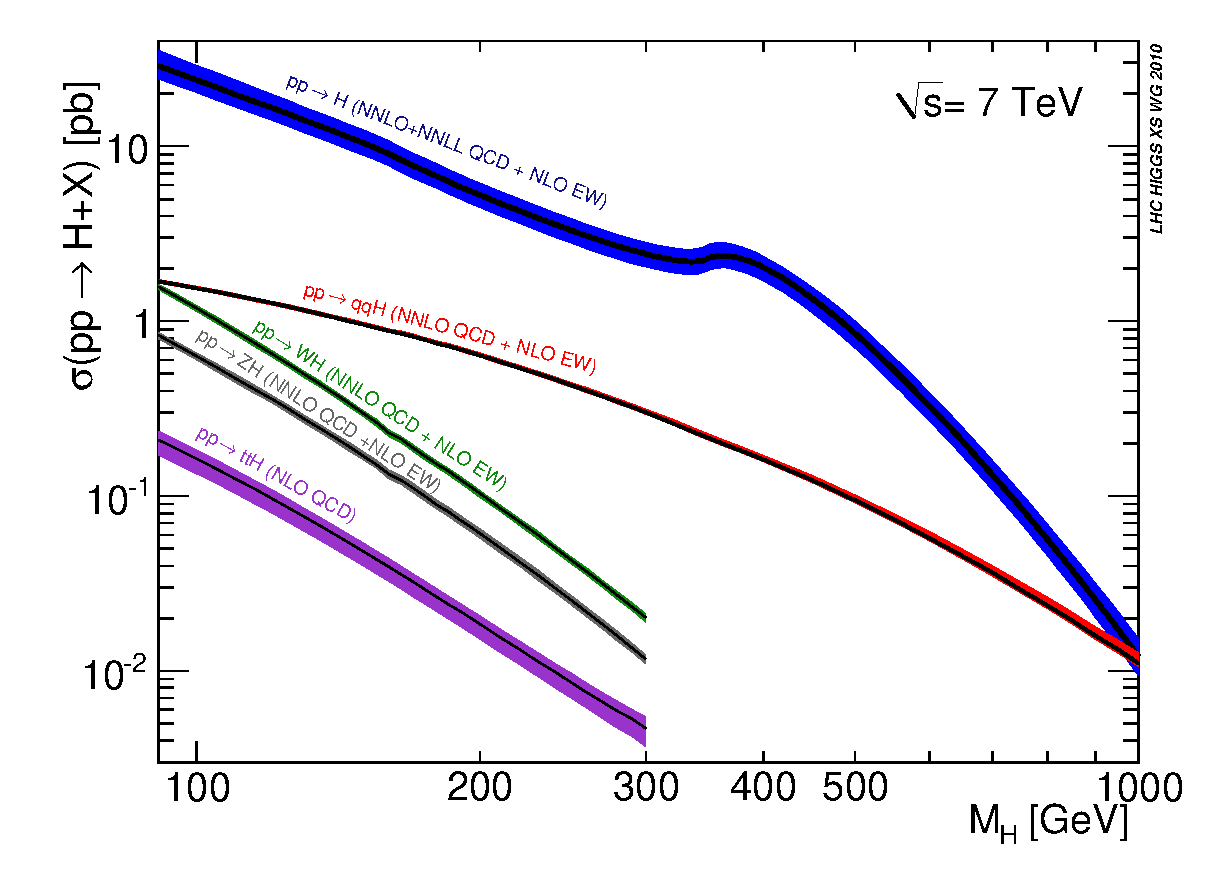
\includegraphics[width=.45\linewidth]{Phenomenology/figures/Higgs_XS_7TeV}
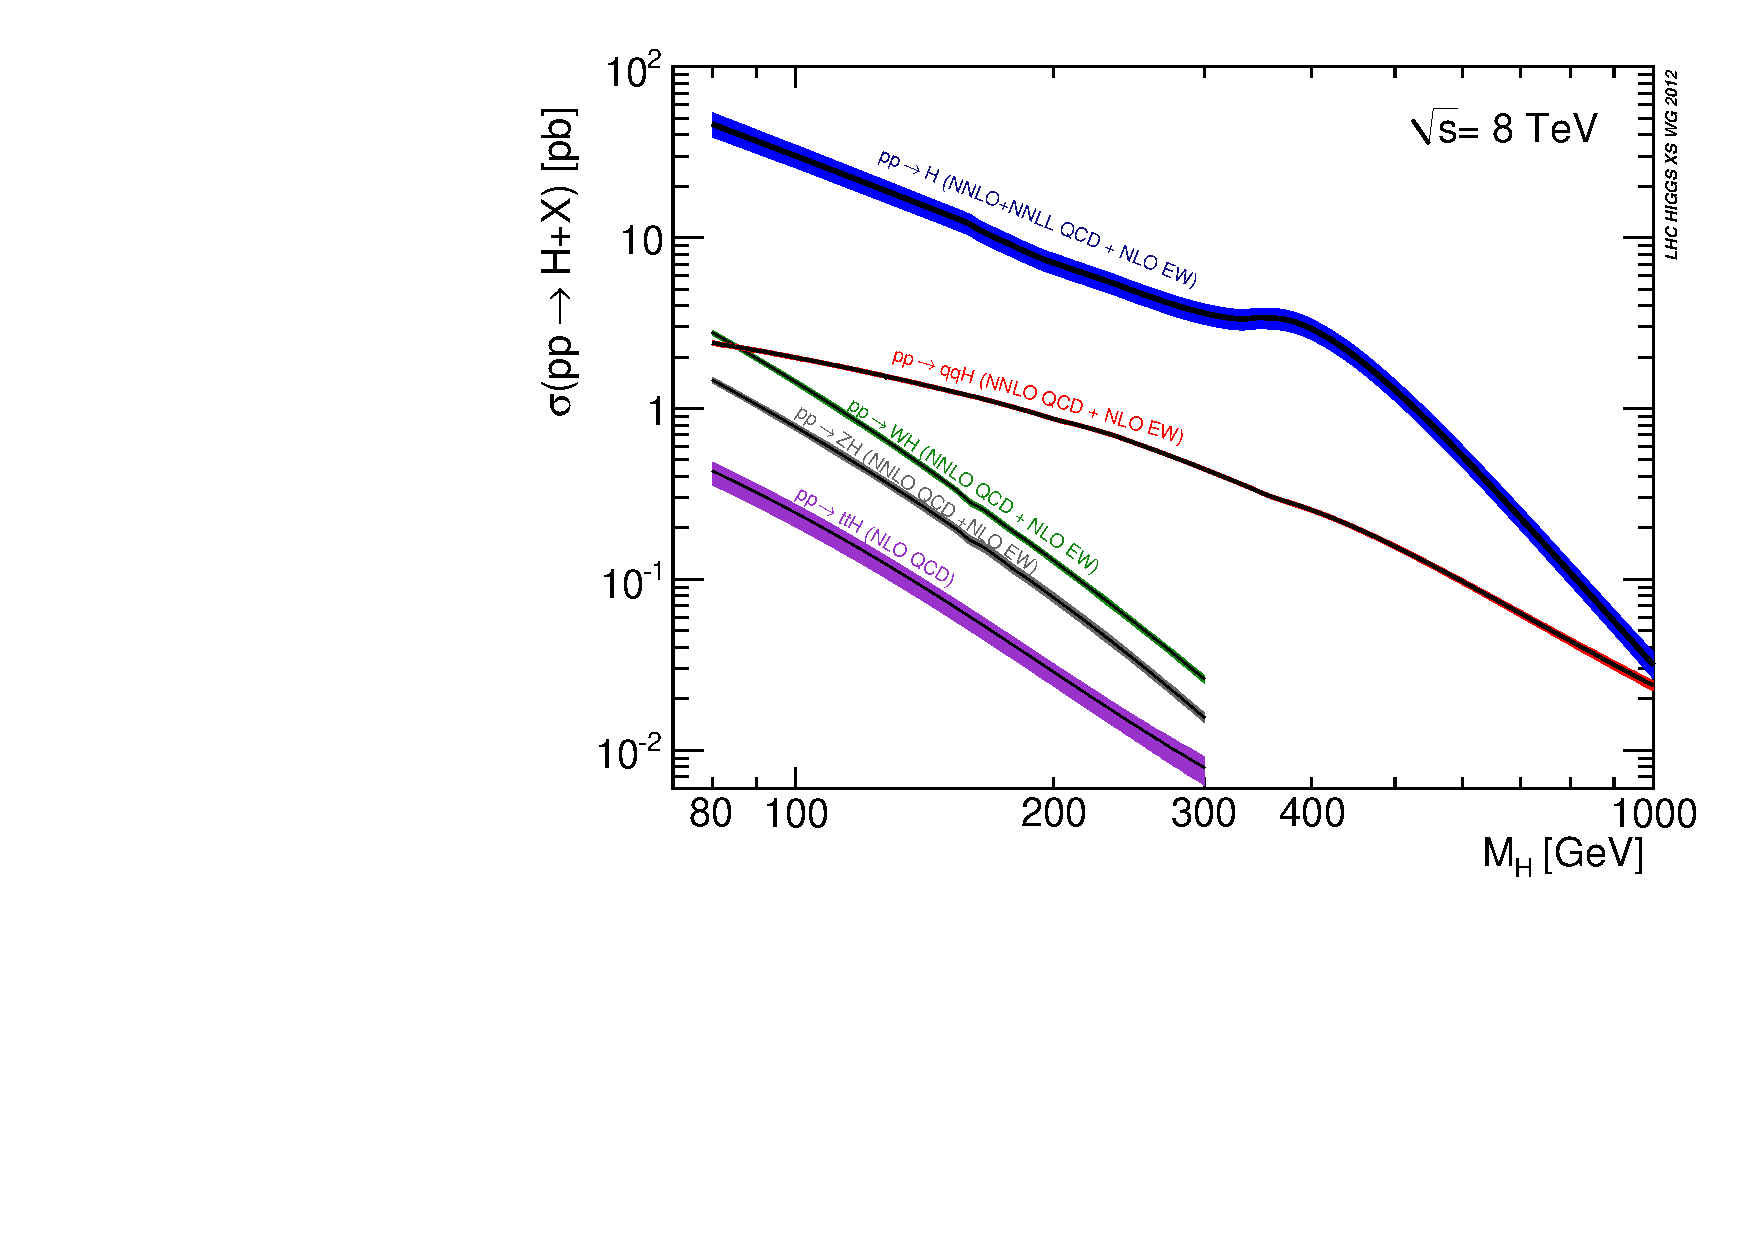
\includegraphics[width=.45\linewidth]{Phenomenology/figures/Higgs_XS_8TeV_lx.pdf}
\caption[Standard Model Production Mechanism of the Higgs at the LHC as a Function of the Higgs' Mass]{SM Cross sections of the different production mechanisms of the Higgs as a function of $m_H$ in the LHC for $\sqrt{s}=$ 7 $\rm{TeV}$ (left) and 8 $\rm{TeV}$ (right) with uncertainty bands~\cite{HXSWG_Properties}. Gluon-gluon fusion (blue) dominates until $m_H \approx 1$ $\rm{TeV}$, where vector boson fusion (red) becomes dominant. WH (green), ZH (grey), and ttH (purple) become energetically unfavorable for higher values of $m_H$.}
\label{fig:HXSWGProduction}
\end{center}
\end{figure}

\subsection{Higgs Decay}
\label{sec:HiggsDecay}

Once the Higgs is produced at LHC, it can decay through any of the allowed channels. Since the SM Higgs couples to both fermions and bosons according to their mass, it can decay at leading order to any pair of massive particles and to massless particles at next-to-leading order via one loop. However, what pair is most favorable depends on the mass of the Higgs, quantified as the \textit{branching ratio} as seen in the left plot of Fig.~\ref{fig:HXSWGDecay}. For $m_H\lesssim2\times m_W$, the Higgs is most likely to decay to a $b\bar{b}$ pair because the $m_b = 4.2 \rm{GeV} \ll m_H$ so the $b$-quarks will be on-shell. For $2\times m_t \gtrsim m_H \gtrsim 2\times m_Z$, $H\rightarrow WW$ and $H\rightarrow ZZ$ can decay to two on-shell bosons, so they become the dominant decays. Lastly, for the highest mass ranges, $m_H \gtrsim 2\times m_t$, the Higgs can also decay to two on-shell top-quarks, so $H\rightarrow t\bar{t}$ becomes much more prevalent. It does not dominate bosonic decay, however, because the fermionic coupling is proportional to the mass of the fermion whereas bosonic coupling is proportional to the square of the mass of the boson.

\begin{figure}[htbp]
\begin{center}
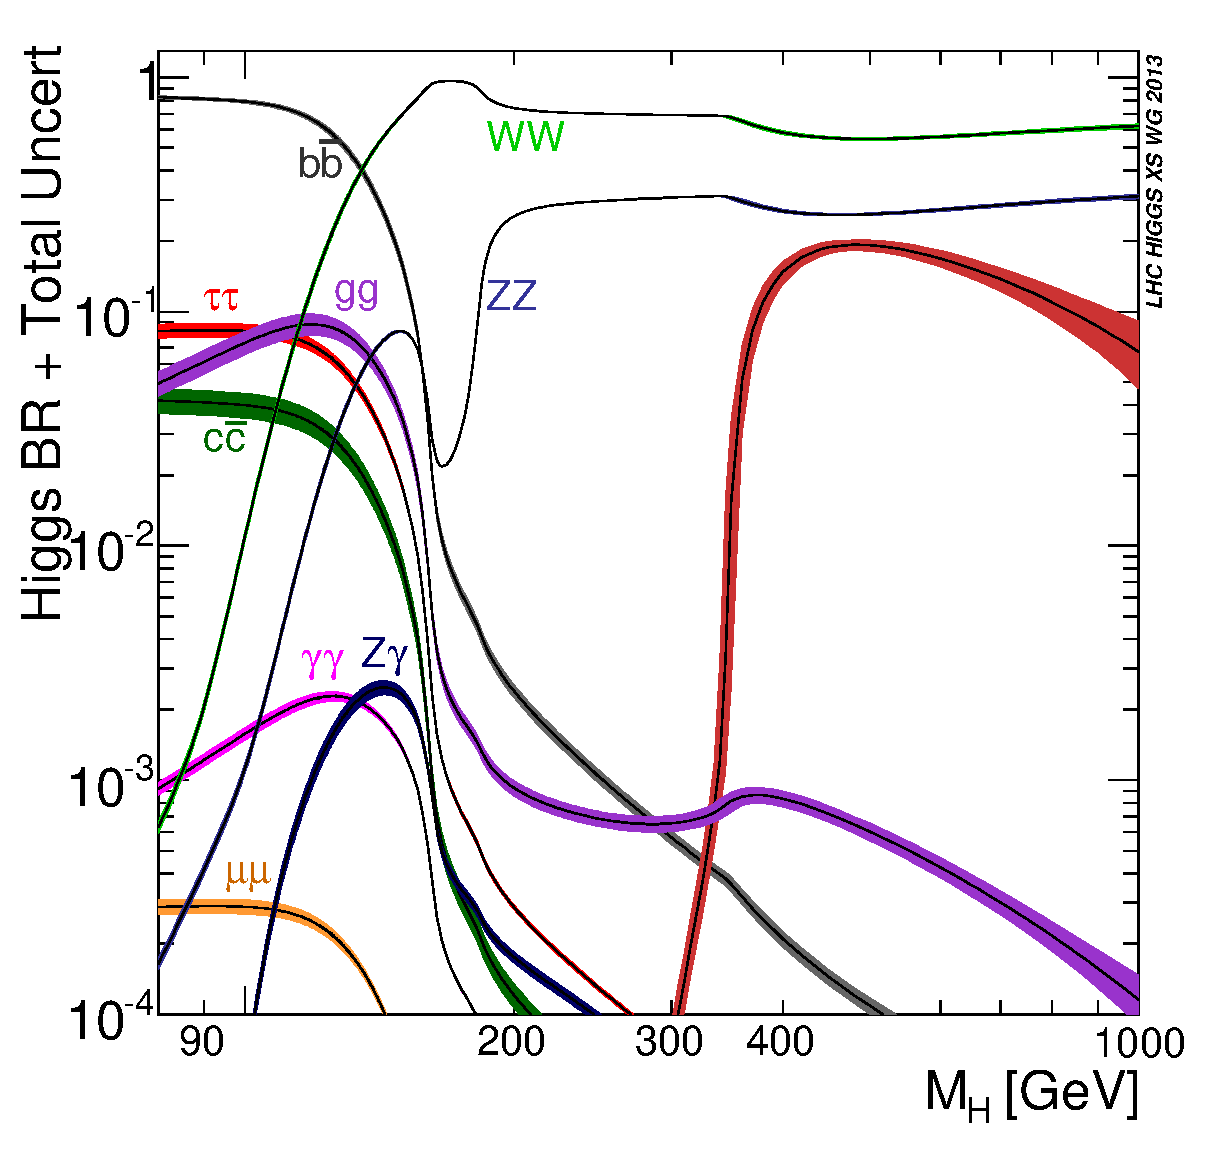
\includegraphics[width=.45\linewidth]{Phenomenology/figures/Higgs_BR}
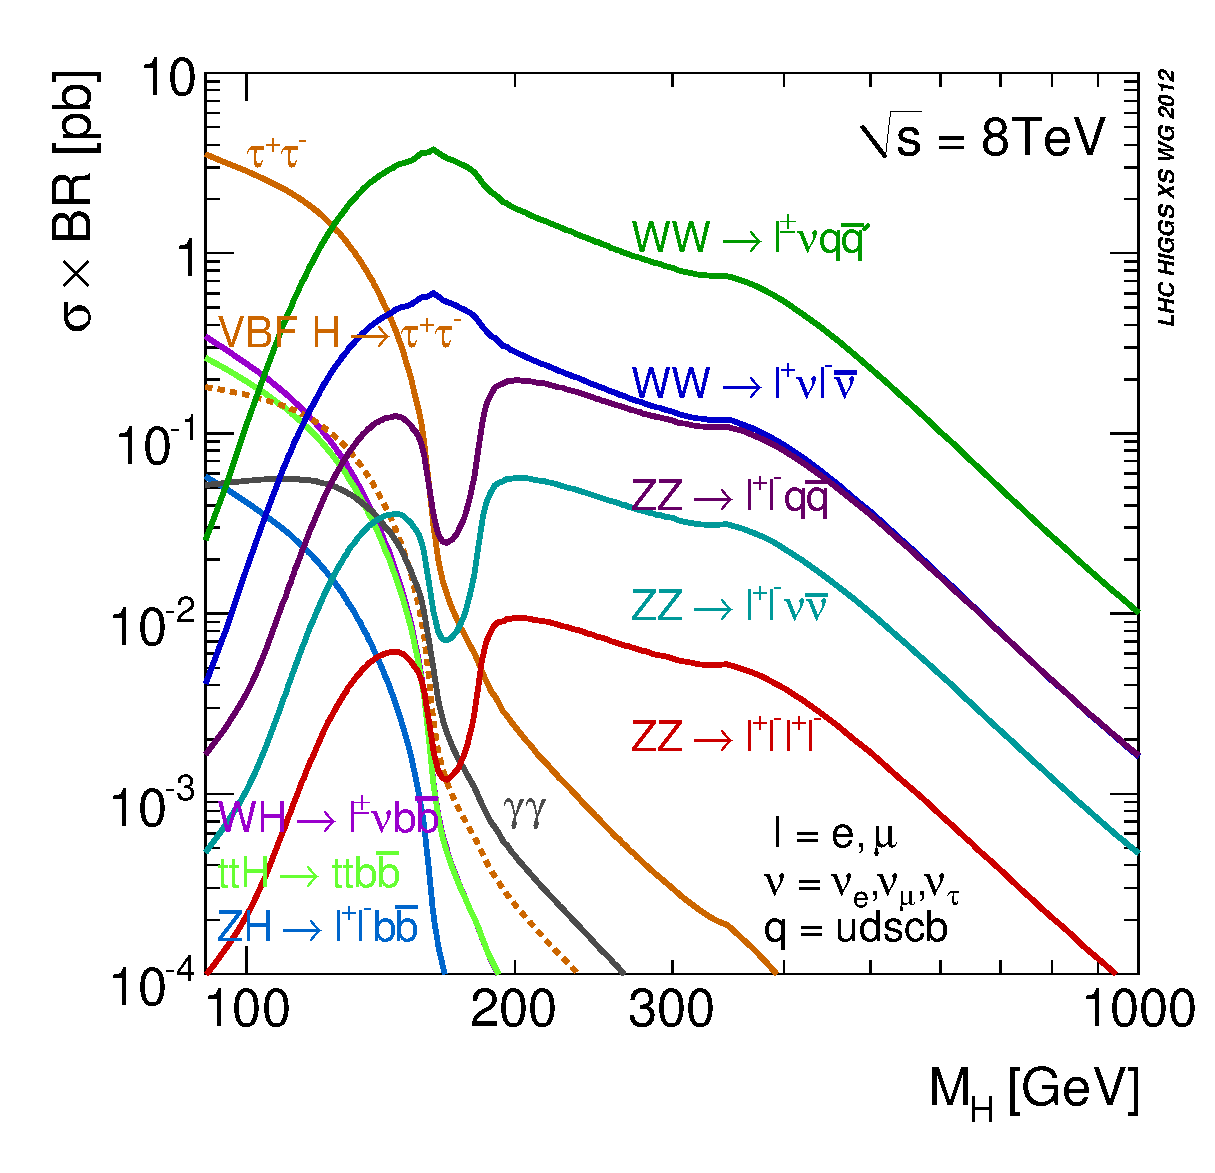
\includegraphics[width=.45\linewidth]{Phenomenology/figures/XSBR_8TeV_SM_HM}
\caption[Standard Model Decay Branching Ratios for the Higgs at the LHC as a Function of the Higgs' Mass]{SM Branching Ratio of the Higgs through different decays with uncertainty bands (left). SM cross sections times branching ratio at the LHC for $\sqrt{s}=$ 8 $\rm{TeV}$ (right).~\cite{HXSWG_Properties}}
\label{fig:HXSWGDecay}
\end{center}
\end{figure}

In CMS, the different analyses of the Higgs are grouped by the final state. For $H\rightarrow \gamma\gamma$ or $H\rightarrow\tau^+\tau^-$, the direct decays of the Higgs are final state. For $H\rightarrow WW$ or $H\rightarrow ZZ$, how the $W$ or $Z$ decays plays a large role in what backgrounds are applicable, so the analyses are further grouped by the decays of the bosons (e.g. $H\rightarrow W^+W^- \rightarrow (l^+\nu)(l^-\nu)$ or $H\rightarrow ZZ \rightarrow (l^+l^-)(q\bar{q})$). In any given Higgs analysis, there are two competing interests: i) maximize the number of expected Higgs events while ii) minimizing the background to increase the overall significance of any signal. The cross sections of the given decay channel as a function of the Higgs mass are displayed in the right plot of Fig.~\ref{fig:HXSWGDecay}.

For most of the valid mass range, $WW\rightarrow l^{\pm}\nu q\bar{q}$ should have the highest number of expected Higgs events. But, any state with quarks in the decay will need to compete with a large background from QCD processes, plus the momentum resolution for jets is not as good as leptons. Furthermore, any decay with neutrinos involves missing energy, meaning that the full kinematics of the $H\rightarrow ZZ\rightarrow 4l$ decay cannot be uniquely determined. For this reason, $ZZ\rightarrow 4l$ is called the ``golden" channel. The full kinematics of the Higgs decay can be accounted for and, using proper cuts, the energy can be measured precisely with comparatively small backgrounds. Although the expected number of Higgs events in this channel will be small, the relative purity makes it ideal for discovery and property measurements of a Higgs boson. 

\section{Studying the $HVV$ Vertex}
\label{sec:HVVVertex}

Roughly speaking, there are two major vertices in the leading order contributions to Higgs production and decay\footnote{By the Feynman rules of the Standard Model, there are a total of five vertices with the Higgs: one Higgs boson and two fermions, one Higgs boson and two bosons, two Higgs bosons and two bosons, three Higgs bosons, and four Higgs bosons. The latter three are all subdominant, and thus beyond the direct scope of this thesis.}: Higgs coupling to two fermions (Hff) or to two bosons (HVV). Of the major production mechanisms from Sec.~\ref{sec:HiggsProduction}, ggF and ttH fall into the former category while VBF and VH fall into the latter. For decay, the $H\rightarrow ZZ \rightarrow 4l$ channel, which we will use in Sec.~\ref{sec:discovery} and~\ref{sec:properties}, involves an HVV vertex. Understanding how this vertex acts in the Standard Model versus a BSM Higgs or background could improve the sensitivity and illuminate what properties of the Higgs could be measured.

\subsection{$H\rightarrow VV$}
\label{sec:HVVDecay}

In the Standard Model, the Higgs boson is a CP-even spin-0 particle. But, as mentioned in Sec.~\ref{sec:findingBSM}, a newly discovered particle could violate CP-symmetry or be spin-2 instead of spin-0: that is, an observed boson may not be the SM Higgs and instead give credence to a BSM theory. For a generic spin-0 resonance $X$ decaying to two spin-1 gauge bosons ($V=Z,$ $W,$ or $\gamma$), the scattering amplitude can be written as~\cite{Gao:2010qx}:
\begin{equation}
  \mathcal{A}(X_{J=0} \rightarrow VV) = \frac{1}{v}\left(g_1m_V^2\epsilon_1^*\epsilon_2^*+g_2f_{\mu\nu}^{*(1)}f^{*(2),\mu\nu}+g_4f_{\mu\nu}^{*(1)}\tilde{f}^{*(2),\mu\nu}\right)
\label{eq:scalarAmp_gform}
\end{equation}
where $v$ is the vacuum expectation value\footnote{The vacuum expectation value is the average value of a parameter in the vacuum, which is non-zero for the Higgs and is plotted in Fig.~\ref{fig:HiggsPotential}. For the Higgs, this value is 246 $\rm{GeV}$.} (VEV) of the SM Higgs field, $g_i$ are the spin-0 couplings with momentum-dependent form factors, $m_V$ is the mass of the boson, $f_{\mu\nu}^{(i)}=\epsilon_i^\mu q_i^\nu - \epsilon_i^\nu q_i^\mu$ is the field strength tensor\footnote{The field strength tensor, $f^{(i)\mu\nu}$, and dual field strength tensor, $\tilde{f}^{*(i)}_{\mu\nu}$, are mathematical representations of the electromagnetic fields in the system.} where $q_i$ is the momentum and $\epsilon_i$ is the polarization vector\footnote{For vector bosons in Electroweak Theory, polarization vectors indicate the orientation of the spin compared to the four-momenta. For each polarization state, the angular distributions of the decay will be limited due to conservation of angular momentum.} of the $i^{th}$ gauge boson, while $\tilde{f}^{(i),\mu\nu}=\frac{1}{2}\epsilon_{\mu\nu\rho\sigma}f^{(i),\rho\sigma}$ is the dual field strength tensor.

In the Standard Model, the Higgs preserves CP-symmetry, which correspond to the $g_1$ and $g_2$ coupling terms. For $m_V \neq 0$, such as $H\rightarrow ZZ$ or $H\rightarrow WW$, $g_1=2i$ at tree-level and is the dominant term while $g_2$ can contribute via radiative corrections (about $10^{-2}$). Clearly, for $m_V=0$, as in $H\rightarrow\gamma\gamma$ or $H\rightarrow gg$, the first term will not contribute so $g_2$ is dominant. The $g_4$ term corresponds to a CP-odd component, where the Higgs would be a pseudoscalar if dominant. For the SM Higgs, $g_4$ is extremely small ($O(10^{-10})$) \cite{Soni:1993} as it only appears at the three-loop level. When the total decay rate is measured independently, as in the case of the $H\rightarrow ZZ \rightarrow 4l$ channel, it is more convenient to use the effective fraction of events to a particular coupling defined as
\begin{equation}
f_{gi} = \frac{|g_i|^2\sigma_i}{|g_1|^2\sigma_1 + |g_2|^2\sigma_2 + |g_4|^2\sigma_4}
\label{eqn:fgi_eqn}
\end{equation}
where $\sigma_i$ is the cross section for the $H\rightarrow VV$ process where $g_i=1,g_{j\neq i}=0$. In general, the $g_i$ couplings can be complex and the phase can be found via $\phi_{gi}=\rm{arg}{(g_i/g_1)}$. Additional amplitudes have been calculated for a spin-1 or spin-2 resonance decaying to two gauge bosons in~\cite{Gao:2010qx}.

For the case when a discovered neutral boson appears to be Higgs-like, i.e. $g_1 \gg g_{2,4}$, the amplitude can be rewritten to emphasize measurements of anomalous couplings compared to the SM predictions. Following the formalism used in~\cite{Gao:2010qx,Bolognesi:2012mm,Anderson:2013afp}, the amplitude can be rewritten as
\begin{equation}
\begin{split}
\mathcal{A}(X_{J=0} \rightarrow VV) = \frac{1}{v}\left(\left[ a_{1}  - e^{i\phi_{\Lambda{Q}}} \frac{\left(q_{1} + q_{2}\right)^{2}}{\left(\Lambda_{Q}\right)^{2}} - e^{i\phi_{\Lambda{1}}} \frac{\left(q_{1}^2 + q_{2}^2\right)}{\left(\Lambda_{1}\right)^{2}}\right]m_{V}^2 \epsilon_{1}^*\epsilon_{2}^*   \right. \\
\left. \vphantom{\frac{\left(q_{1} + q_{2}\right)^{2}}{\left(\Lambda_{Q}\right)^{2}}} + a_{2}^{}  f_{\mu \nu}^{*(1)}f^{*(2),\mu\nu} 
+ a_{3}^{}   f^{*(1)}_{\mu \nu} {\tilde f}^{*(2),\mu\nu}\right)
\end{split}
\label{eq:scalarAmpl_wformfactors}
\end{equation}
where the momentum dependence in the $a_1$ term is explicitly defined. $\Lambda$ and $\Lambda_{Q}$ are the mass scales of BSM physics and $\phi_{\Lambda{1}}$ and $\phi_{\Lambda{Q}}$ are the phases of their respective terms. The $\Lambda_1$ term corresponds to new, not yet observed particles contributing to the $HVV$ vertex while $\Lambda_Q$ corresponds to the $H\rightarrow VV$ interaction having an overall momentum dependence such that there could be enhancement of the Higgs off-shell. Eqn.~(\ref{eqn:fgi_eqn}) can then be rewritten as the equations
\begin{align}
f_{ai} &= \frac{|a_i|^2\sigma_i}{|a_1|^2\sigma_1 + |a_2|^2\sigma_2 + |a_4|^2\sigma_4 + \sigma_{\Lambda_{1}}/(\Lambda_1)^4} \label{eqn:fai} \\
f_{\Lambda{1}} &= \frac{\sigma_{\Lambda_{1}}/(\Lambda_1)^4}{|a_1|^2\sigma_1 + |a_2|^2\sigma_2 + |a_4|^2\sigma_4 + \sigma_{\Lambda_{1}}/(\Lambda_1)^4} \label{eqn:fL1} \\
f_{\Lambda{Q}} &= \frac{\tilde{\sigma}_{\Lambda{Q}}/\left(\Lambda_Q\right)^4}{|a_1|^2\sigma_1 + \tilde{\sigma}_{\Lambda{Q}}/\left(\Lambda_Q\right)^4} \label{eqn:fLQ}
\end{align}
with $\sigma_i$ still corresponding to the respective cross sections for Eqns.~(\ref{eqn:fai}) and (\ref{eqn:fL1}), as it is in Eqn.~(\ref{eqn:fgi_eqn}). For Eqn.~(\ref{eqn:fLQ}), since $f_{\Lambda{Q}}$ can only be measured by comparing on-shell and off-shell, $\sigma_1$ now refers to the total on-shell cross section where $\tilde{\sigma}_{\Lambda{Q}}/\sigma_{1}=m_{H}^4$.

But how do these coupling ratios manifest in the observation of a resonance? In Eqn.~(\ref{eq:scalarAmpl_wformfactors}), there is clear dependence on the polarization vectors of the decay bosons. As detailed in~\cite{Gao:2010qx}, by conservation of angular momentum, the spin of the resonance restricts the allowed polarization vectors and thus the helicity amplitudes which can determine the angular distributions. In other words, for the SM Higgs, the spins of the decay gauge bosons are correlated which will have direct impact on the likely angular distributions of the final decay state. These expected distributions, derived directly from the matrix element, can be used to assign probabilities on an event-by-event basis to discriminate between the SM Higgs and a BSM model or between the SM Higgs and background.

For the generic $X\rightarrow VV \rightarrow 4f$ decay channel, in the rest frame of the resonance nine parameters are sufficient to fully characterize the kinematics: three masses ($m_X$, $m_{V1}$, $m_{V2}$) and six angles. Figure~\ref{fig:HVVAngles} shows five of these angles, with a final global rotation about the beam line making the sixth. The five angles in Fig.~\ref{fig:HVVAngles}, referred to collectively as $\vec{\Omega}$, are all influenced by the helicity distributions from the amplitude listed above. For $m_X > 2\times m_V$, both of the gauge bosons will be on-shell. But if $m_X < 2\times m_V$ then the only way this decay can be observed is if at least one of the gauge bosons are off-shell. The global rotation along with the spatial momentum of the resonance are not influenced by the spin-parity of the state, so they don't aid in discriminating between different models, although the spatial momentum assists in separation of production mechanisms.

\begin{figure}[htbp]
\begin{center}
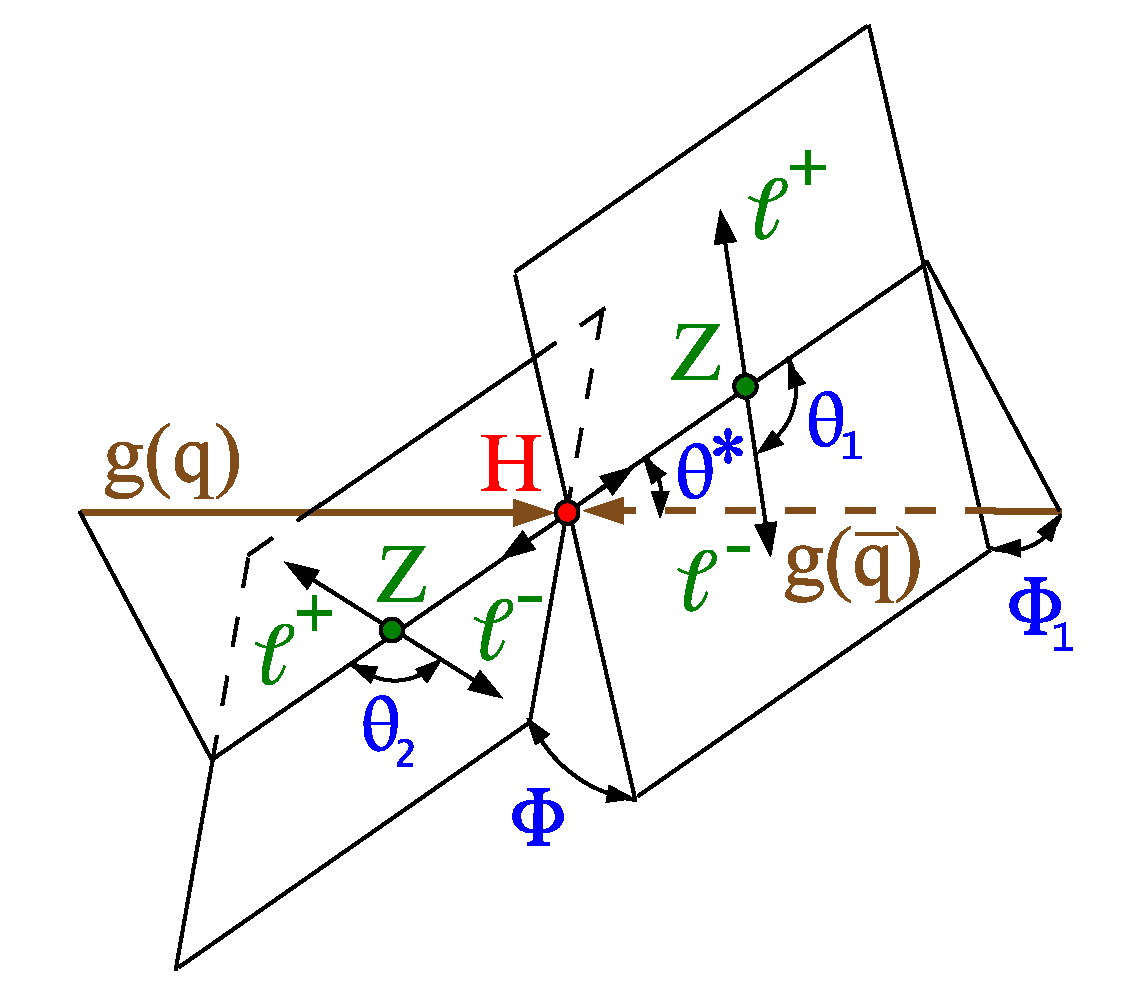
\includegraphics[width=.5\linewidth]{Phenomenology/figures/angles-HZZ4l.eps}
\caption[Definition of Angles in $H\rightarrow VV$ Decay]{Angles in the $H\rightarrow ZZ \rightarrow 4l$ decay as defined in the Higgs rest frame. Brown lines indicate incoming gluons or quarks along beam line. $\theta^*$ defines the angle from beam line to the decay line of the $Z$ bosons. $\Phi$ and $\Phi_1$ define the orientation of the planes for each $Z\rightarrow l^+l^-$ decay relative to the $H \rightarrow ZZ$ decay. $\theta_1$ and $\theta_2$ are the angles of the leptonic decay lines to the $Z_{1,2}$ momenta.}
\label{fig:HVVAngles}
\end{center}
\end{figure}

As stated in Sec.~\ref{sec:HiggsDecay}, the $ZZ\rightarrow 4l$ final state allows for precise and complete calculation of the decay kinematics, so this matrix element approach is ideal for Higgs searches of this final state. To discriminate background or alternative signals from the SM Higgs, there are two methods to analyze the three masses and five relevant angles of the decay kinematics on an event-by-event basis. A full 8D multidimensional fit could be used~\cite{Chen:2014pia}, but a very large number of events are required to properly populate the distributions, making it both computationally expensive and mostly inaccessible to decays with small yields. Alternatively, a single kinematic discriminant could be constructed where the information from the distributions is compounded into unified probabilities. This is the \textit{matrix element likelihood approach} (MELA)~\cite{Gao:2010qx,Bolognesi:2012mm} which is used in CMS $ZZ\rightarrow 4l$ analyses.

Discriminants in MELA are built from probabilities, using the equation
\begin{equation}
\mathcal{D} = \frac{\mathcal{P}_{\rm{sig}}}{\mathcal{P}_{\rm{sig}} + \mathcal{P}_{\rm{bkg}}} = \left[1+ \frac{\mathcal{P}_{\rm{bkg}}(m_{4l};m_1,m_2,\vec{\Omega})}{\mathcal{P}_{\rm{sig}}(m_{4l};m_1,m_2,\vec{\Omega})}\right]^{-1}
\label{eq:MELADisc}
\end{equation}
where $\mathcal{P}_{\rm{bkg}}$ could refer to the probability from the dominant background in the analysis or an alternative signal hypothesis (e.g. a pseudoscalar Higgs) and $\mathcal{P}_{\rm{sig}}$ usually refers to the probability of the SM Higgs, though other signals could be used. Each probability ideally stems from an analytic matrix element, as is described in Eqn.~\ref{eq:scalarAmpl_wformfactors}, but when unavailable MC simulation can be used to populate the probability distributions. To account for this, the \textsc{JHU} generator (\textsc{JHUGen}) was written.

\textsc{JHUGen} is a dedicated MC generator, which full encodes the correlations and amplitudes of Eqn.~\ref{eq:scalarAmpl_wformfactors} as well as analogous amplitudes for spin-1 and spin-2 resonances. For $X\rightarrow VV$ decay, these matrix elements can be used in event generation or directly for building discriminants. Both properties will be utilized in the Higgs discovery (Sec.~\ref{sec:discovery}) and properties measurements (Sec.~\ref{sec:properties}). Comparisons of a few angular distributions from the analytic matrix element and the events from \textsc{JHUGen} are found in ~\cite{Bolognesi:2012mm}.

\subsection{$VV \rightarrow H$}
\label{sec:VBFVertex}

\begin{figure}[htbp]
\begin{center}
\unitlength=1mm
\subfloat{
\begin{fmffile}{Phenomenology/figures/HVVVertex}
\begin{fmfgraph*}(40,40)
  \fmfleft{i1}
  \fmfright{sp1,sp2}
  \fmf{dashes,label=$H$}{i1,v0}
  \fmf{photon,label=$V$}{v0,sp2}
  \fmf{photon,label=$V$}{v0,sp1}
\end{fmfgraph*}
\end{fmffile}
}
\subfloat{
\begin{fmffile}{Phenomenology/figures/VVHVertex}
\begin{fmfgraph*}(40,40)
  \fmfleft{i1,i2}
  \fmfright{sp1}
  \fmf{photon,label=$V$}{i1,v0}
  \fmf{photon,label=$V$}{i2,v0}
  \fmf{dashes,label=$H$}{v0,sp1}
\end{fmfgraph*}
\end{fmffile}
}
\caption[Feynman Diagrams of the HVV vertex]{On left, the Higgs decays to two gauge bosons. On the right, two gauge bosons produce the Higgs. Any calculation of the amplitude of one vertex will be identical to the calculation of the time reversed vertex.}
\label{fig:HVVVertex}
\end{center}
\end{figure}

When looking at the $HVV$ vertex in Fig.~\ref{fig:HVVVertex}, it becomes obvious that $VV\rightarrow H$ is just a time reversal of the $H\rightarrow VV$ decay. The clear benefit is that, because the diagrams used to form the amplitude in Eqn.~\ref{eq:scalarAmp_gform} are identical, the end result is the same. The mathematical description provided by the matrix element approach in Sec.~\ref{sec:HVVDecay} applies to VBF production as well, with a few key differences:

\begin{description}
\item[Production v Decay Kinematics] \hfill \\
For VBF, the production kinematics are seen in Fig.~\ref{fig:VBFAngles}. For $H\rightarrow ZZ \rightarrow 4l$ decay, the kinematics of the decay can be fully defined using the three masses and five decay angles which can all be fully reconstructed. VBF is considerably more complicated as i) the direction and momentum fraction of the incoming partons are tied to the parton distribution function and ii) the production bosons transfer momentum from these incoming quarks.
\item[Universality of Decay Channel] \hfill \\
Although VBF is the subdominant production mechanism, it exists for every decay channel. Thus, measurements of the $HVV$ vertex can be combined across multiple analyses to improve overall performance.
\item[High Mass Sensitivity] \hfill \\
As the mass of the Higgs increases, VBF production becomes more and more likely. Any searches for high mass resonances should be tuned to emphasize VBF production.
\item[Cross Section Differences] \hfill \\
In Eqn.~(\ref{eqn:fai}), there is dependence on the anomalous cross section. Because of the large off-shell mass of $V^*$ in production, the ratio of anomalous cross section to SM cross section is considerably higher than in $H\rightarrow ZZ$ decay, allowing for higher precision with fewer events.
\end{description}

\begin{figure}[htbp]
\begin{center}
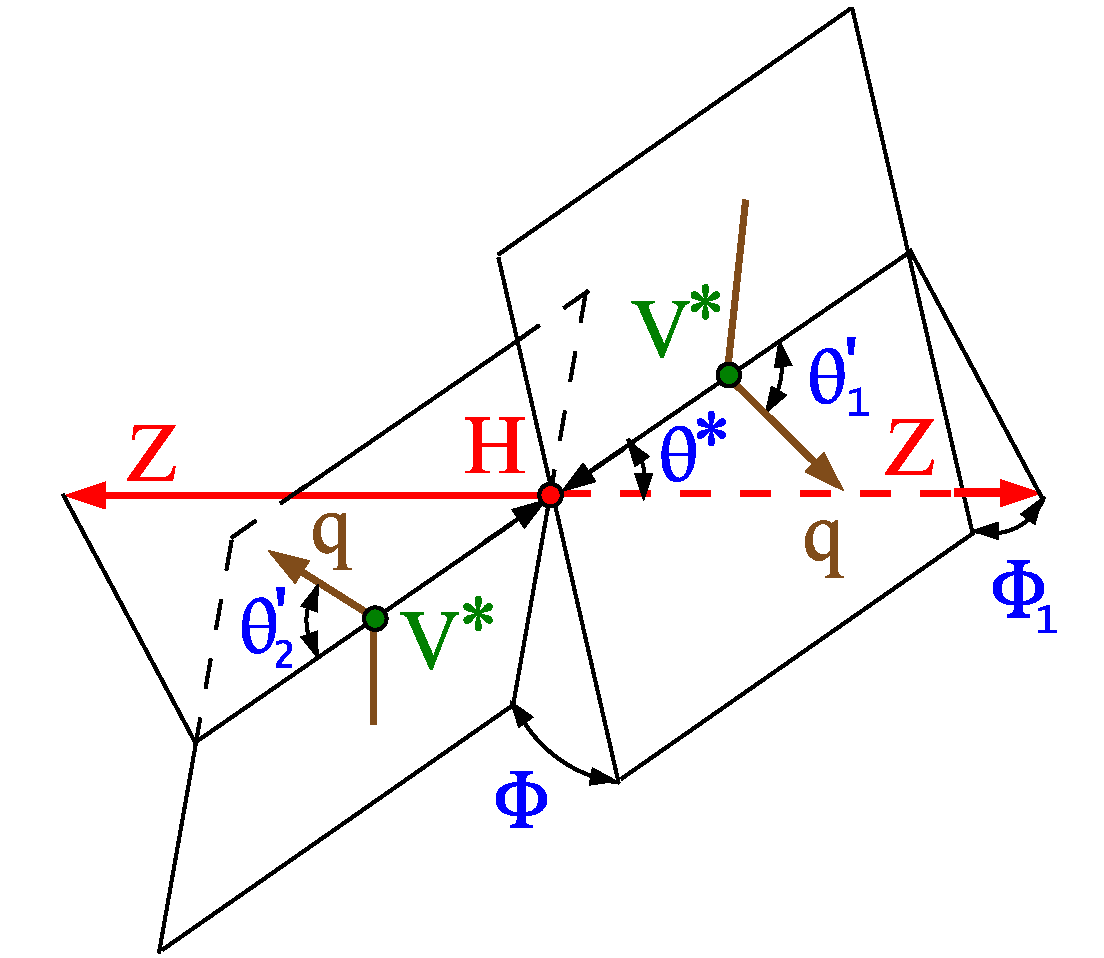
\includegraphics[width=.5\linewidth]{Phenomenology/figures/angles-HZZVBF_cms.pdf}
\caption[Definition of Angles in VBF Production]{Angles of VBF production in $H\rightarrow ZZ$. Compared to Fig.~\ref{fig:HVVAngles}, the angles mostly have similar definitions, but time reversed. The masses $m_{1,2}$ in decay are analogous to the  of the virtual $V^*$ bosons in production while $\theta_1^{'}$ and $\theta_2^{'}$ are analogous to $\theta_1$ and $\theta_2$, but the momentum lines for the incoming and outgoing quarks are not collinear.}
\label{fig:VBFAngles}
\end{center}
\end{figure}

Many BSM models predict multiple Higgs bosons of varying spin states. VBF production is crucial both to unambiguously discover new BSM particles across multiple decay channels and to use the $XVV$ vertex to measure the spin-parity state of any discovered resonance. Roughly speaking, although the full kinematics of the production are limited, the two jets that come from VBF production should have a wide forward-backward separation ($\Delta\eta$) and a large invariant mass of the dijet pair ($m_{JJ}$). Further correlations between these jets and the resonance can both illuminate its spin-parity and aid in the background separation. A numerical computation of the VBF matrix element is available in \textsc{JHUGen}, both for generation of events and calculation of probabilities for discriminants.

\subsection{$V^* \rightarrow VH$}
\label{sec:VHVertex}

Lastly, the $HVV$ vertex can be studied looking at Higgs-strahlung production. As with VBF in Sec.~\ref{sec:VBFVertex}, the mathematics of the generic amplitude in Eqn.~\ref{eq:scalarAmp_gform} are identical. In fact, if the final state $V$ boson decays to a jet pair, the decay products are also identical to VBF. However, where VBF expects a pair of strongly separated jets with a large invariant mass, the jet pair in VH production should have an invariant dijet mass, $m_{JJ}$, close to the on-shell mass of the $V$ boson. Modeling this with a gaussian\footnote{$m_{JJ}$ will be close to $m_V$, but resolution effects in the detector will smear out the true mass distribution.} about the expected $m_V$, the remaining kinematics can be used to build a probability. Although VH also depends on the parton distribution function, because the four-momentum of the VH pair can be well constructed and the incoming partons directly produce the virtual $V^*$, an analytic form of the matrix element is constructed and can be used in Higgs analyses.

\section{Summary}
\label{sec:pheno_summary}

Looking through the possible Higgs decay channels, analyzing in the $ZZ \rightarrow 4l$ decay channel is clearly a powerful method to search for the Higgs boson. By relying on the precise resolution for leptons in CMS, any $ZZ \rightarrow 4l$ event can be fully reconstructed. Then, these detailed kinematics can be used both in the search for the Higgs boson when comparing to backgrounds or in the measurement of its properties. In Sec.~\ref{sec:discovery}, we will use the techniques listed above to search for a Higgs boson. Then, in Sec.~\ref{sec:properties}, we will extract what the properties of this new boson are and whether it agrees with Standard Model expectations.
